% This file was created by matplotlib2tikz v0.7.4.
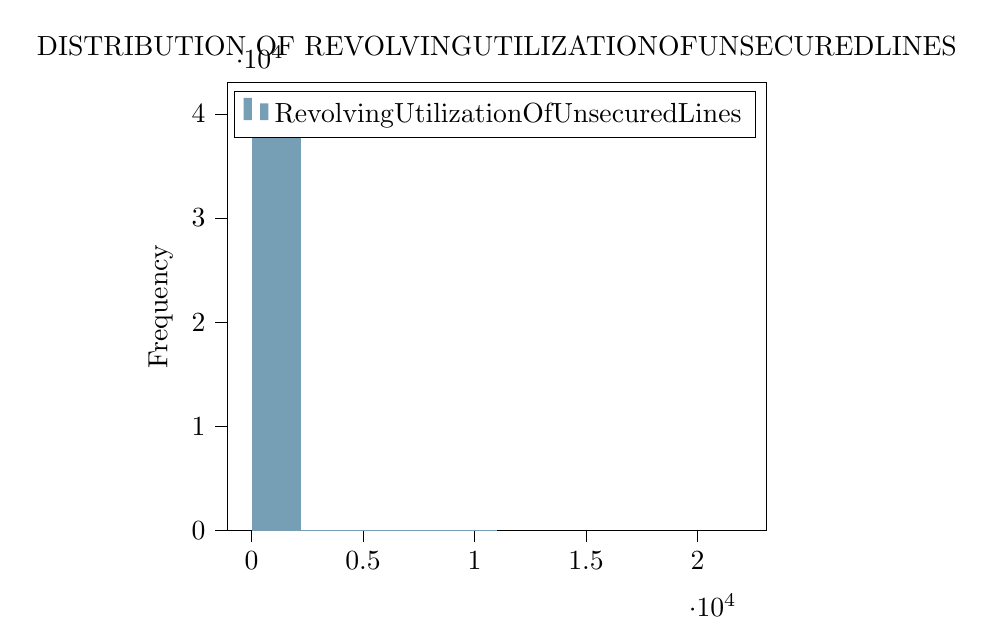
\begin{tikzpicture}

\definecolor{color0}{rgb}{0.462745098039216,0.623529411764706,0.713725490196078}

\begin{axis}[
tick align=outside,
tick pos=left,
title={\printsubsection{\MakeUppercase{Distribution of RevolvingUtilizationOfUnsecuredLines}}},
x grid style={white!69.01960784313725!black},
xmin=-1100, xmax=23100,
xtick style={color=black},
y grid style={white!69.01960784313725!black},
ylabel={Frequency},
ymin=0, ymax=43034.25,
ytick style={color=black}
]
\draw[fill=color0,draw opacity=0] (axis cs:0,0) rectangle (axis cs:2200,40985);
\addlegendimage{ybar,ybar legend,fill=color0,draw opacity=0};
\addlegendentry{RevolvingUtilizationOfUnsecuredLines}

\draw[fill=color0,draw opacity=0] (axis cs:2200,0) rectangle (axis cs:4400,14);
\draw[fill=color0,draw opacity=0] (axis cs:4400,0) rectangle (axis cs:6600,6);
\draw[fill=color0,draw opacity=0] (axis cs:6600,0) rectangle (axis cs:8800,5);
\draw[fill=color0,draw opacity=0] (axis cs:8800,0) rectangle (axis cs:11000,2);
\draw[fill=color0,draw opacity=0] (axis cs:11000,0) rectangle (axis cs:13200,1);
\draw[fill=color0,draw opacity=0] (axis cs:13200,0) rectangle (axis cs:15400,1);
\draw[fill=color0,draw opacity=0] (axis cs:15400,0) rectangle (axis cs:17600,0);
\draw[fill=color0,draw opacity=0] (axis cs:17600,0) rectangle (axis cs:19800,1);
\draw[fill=color0,draw opacity=0] (axis cs:19800,0) rectangle (axis cs:22000,1);
\end{axis}

\end{tikzpicture}